\documentclass{standalone}
\usepackage{tikz}
\usetikzlibrary{arrows.meta}
\tikzset{label/.style = {inner sep=1pt, fill=white}}
%\tikzset{nd/.style={circle, inner sep=0pt}}
\tikzset{nd/.style={inner sep=1pt}}
\tikzset{>=Latex}
\tikzset{arc/.style = {->, semithick, >=Latex}}
\begin{document}
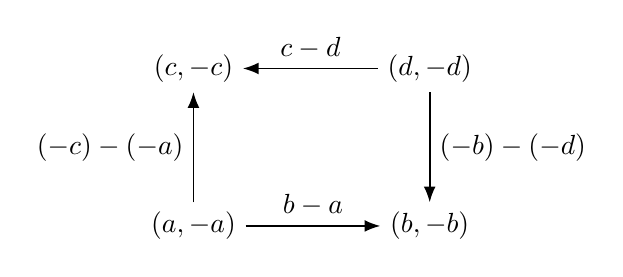
\begin{tikzpicture}
    \node (bl) at (0,0) {$(a,-a)$};
    \node (br) at (3,0) {$(b,-b)$};
    \node (tl) at (0,2) {$(c,-c)$};
    \node (tr) at (3,2) {$(d,-d)$};
    \draw[arc] (bl) to node[above] {$b-a$} (br);
    \draw[arc] (tr) to node[above] {$c-d$} (tl);
    \draw[arc] (tr) to node[right] {$(-b)-(-d)$} (br);
    \draw[arc] (bl) to node[left] {$(-c)-(-a)$} (tl);
\end{tikzpicture}
\end{document}